\section{Technical acknowledgements}
\paragraph{}
The following code presented was written using \emph{R}. The images from which the shapes were extracted were used as gray images. \ref{fig:gray-images}

\section{Loading data}
\paragraph{}
Images are loaded then converted to grayscale. Right now, we are not interested in their color, so they'll only be black and white.

\begin{lstlisting}[language=R, caption=Loading images in R]
    rdfReadGreyImage <- function (nom) {
        image <- readImage (paste('images/', nom, sep=''))
        if (length (dim (image)) == 2) {
            image
        } else {
            channel (image, 'red')
        }
    }
\end{lstlisting}

\begin{figure}[h]
    \centering
    
\includegraphics[scale=2.0]{rdf-carre-6.png}
    
\includegraphics[scale=2.0]{rdf-carre-10.png}
    
\includegraphics[scale=2.0]{rdf-carre-10-30deg.png}
    
\includegraphics[scale=2.0]{rdf-triangle-10-15deg.png}
    
\includegraphics[scale=2.0]{rdf-triangle-10-45deg.png}
    
\includegraphics[scale=2.0]{rdf-triangle-10-60deg.png}
    
\includegraphics[scale=2.0]{rdf-triangle-20.png}
    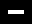
\includegraphics[scale=2.0]{rdf-rectangle-horizontal.png}
    
\includegraphics[scale=2.0]{rdf-rectangle-vertical.png}
    
\includegraphics[scale=2.0]{rdf-rectangle-diagonal.png}
    \caption{Shape images}
    \label{fig:gray-images}
\end{figure}

\clearpage

\section{Moments of a shape}
\paragraph{}
We define the \emph{moment of a shape} as the following:
$$M_{ij} = \sum_{x}\sum_{y} x^{i} y^{j} A(x, y)$$
\paragraph{}
where $A(x, y)$ is the value of the pixel $(x, y)$ of the shape's image. One can easily observe that $M_{00}$ is equal to the number of pixels that are not black. We call that the \emph{surface} of the shape.

\begin{lstlisting}[language=R, caption=Calculating the moment of a shape]
    rdfMoment <- function (im, p, q) {
        x <- (1 : (dim (im)[1])) ^ p
        y <- (1 : (dim (im)[2])) ^ q
        as.numeric (rbind (x) %*% im %*% cbind (y))
        }
\end{lstlisting}

\paragraph{}
The \emph{barycenter} is defined as being the following:
$$(\bar{x}, \bar{y}) = (\frac{M_{10}} {M_{00}}, \frac{M_{01}} {M_{00}})$$

\paragraph{}
Having these, we can now make our $M_{ij}$ invariant to the translation of the shape. We can define the \emph{centered moment} as being:
$$\mu_{ij} = \sum_{x}\sum_{y} (x - \bar{x})^i(y - \bar{y})^j I(x, y)$$

\begin{lstlisting}[language=R, caption=Calculating centered moments]
    rdfMomentCentre <- function (im, p, q) {
        # Barycentre
        s <- rdfSurface (im)
        cx <- rdfMoment (im, 1, 0) / s
        cy <- rdfMoment (im, 0, 1) / s
        # Initialiser les vecteurs x et y
        x <- (1 : (dim (im)[1]) - cx) ^ p
        y <- (1 : (dim (im)[2]) - cy) ^ q
        # Calcul du moment centre
        as.numeric (rbind (x) %*% im %*% cbind (y))
      }
      
\end{lstlisting}

% -----------------------------------------------
\section{Inertia matrix}
\paragraph{}
Inspiring ourselves from physics, we may use these moments to calculate the inertia matrix:
$$ I = 
\begin{pmatrix}
    \mu_{20} & \mu_{11}\\
    \mu_{11} & \mu_{02}
\end{pmatrix}
$$

\clearpage
% -----------------------------------------------
\paragraph{}
We'll be using $I$ later on to tell which is the main axis of inertia for different shapes.
For now, let's take a look at its values for the images with rectangles and squares.
\begin{figure}[H]
    \centering
    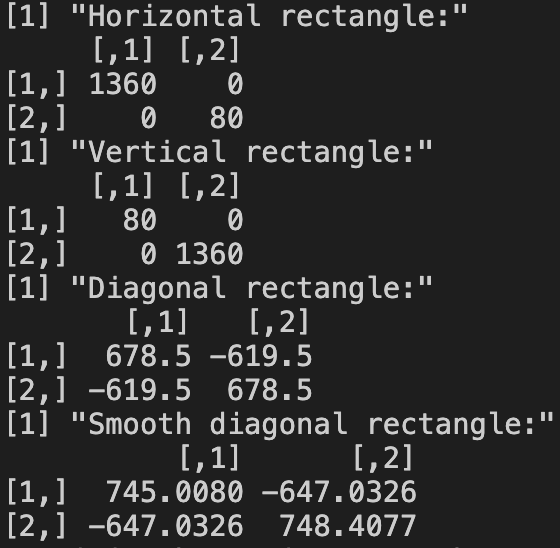
\includegraphics[height=5cm]{rectangles-moments.png}
    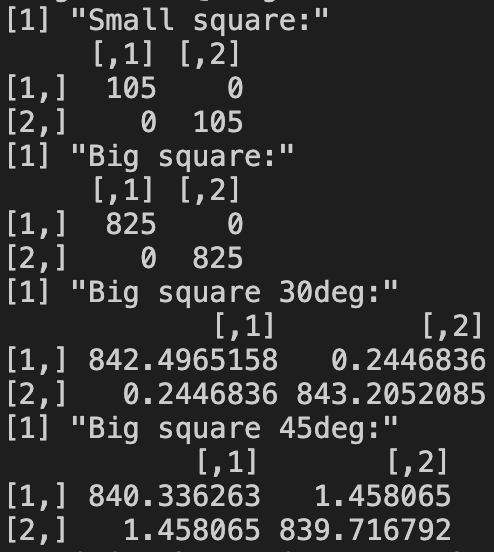
\includegraphics[height=5cm]{squares-moments.png}
    \caption{Inertia matrices for rectangles and squares}
\end{figure}
\paragraph{}
Upon calculating the values for the rectangles, we can observe that their matrix of inertia is different for each shape.
For the horizontal rectangle, it's intuitive that the following equation should happen: $\mu_{20} > \mu_{02}$.
That's because there are more pixels distributed over the $x$ axis. For the vertical rectangle, it's the opposite.
The inertia matrix tells us just that.
For the diagonal rectangle, there's an interesting observation: $\mu_{20} = \mu_{02}$. That's because the rectangle is rotated at 45 degrees, so the pixels are uniformely distributed horizontally and vertically.
For the two diagonal rectangles, the values differ, but it's interesting to notice that the proportion $\frac{\mu_{20}}{\mu_{02}}$ is about the same. That would mean that the rectangles are similarly oriented, which is true.
\paragraph{}
The $\frac{\mu_{20}}{\mu_{02}}$ proportion is also kept in the case of the the squares which aren't rotated.
Another interesting observation is that for the shapes that aren't rotated, $\mu_{11} = 0$.
All of these already give us valuable information as to how the shape looks, so they can definitely be used as shape attributes.
However, we can still improve these.
% -----------------------------------------------

\section{Shape's inertia}
\subsection{Normalised Moment Centers}
\paragraph{}
For our next trick, we can make $\mu_{ij}$ invariant to the scale of the image. We define the \emph{normalized centered moment} as the following:
$$\eta_{ij} = \frac{\mu_{ij}}{\mu_{00}^{1 + \frac{i + j}{2}}}$$

\begin{lstlisting}[language=R, caption=Calculating normalised centered moments]
    rdfMomentCentreNormalise <- function (img, p, q){
        upq = rdfMomentCentre(img, p, q)
        u00 = rdfMomentCentre(img, 0, 0)
        normalised = upq / (u00 ** (1 + (p + q)/2))
        normalised
    }
\end{lstlisting}

\clearpage

\paragraph{}
Taking a look at the values\footnote{The values were rounded to 3 decimals}, we can notice that $\eta_{22}$, for example, becomes invariant to the size of the image (for example for the triangles).
$\eta_{20}$ and $\eta_{02}$ still tell us how pixels are distributed over the $x$ and $y$ axis, but they are now not influenced by the shape's size.

\begin{figure}[h]
    \centering
    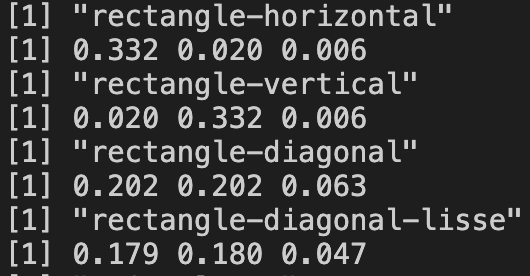
\includegraphics[width=5cm, height=5cm]{rectangles_normalised_moments.png}
    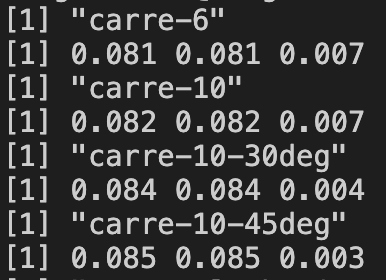
\includegraphics[width=5cm, height=5cm]{squares_normalised_moments.png}
    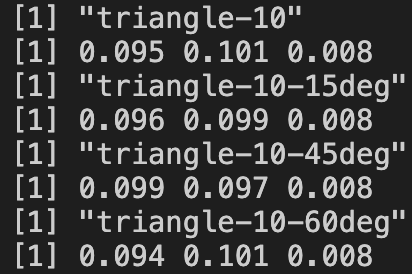
\includegraphics[width=5cm, height=5cm]{triangles_normalised_moments.png}
    \caption{Normalised moment centers}
\end{figure}

\subsection{Main moments of inertia}
\paragraph{}
Using the \emph{normalised centered moments}, rather than just \emph{centered moments}, we can calculate:
$$ I = 
\begin{pmatrix}
    \eta_{20} & \eta_{11}\\
    \eta_{11} & \eta_{02}
\end{pmatrix}
$$
\paragraph{}
Afterwards, we can calculate the \emph{eigen values} of the matrix $I$. The values obtained, $I_1$ and $I_2$ are the \emph{main moments of inertia}:
$$ I' = 
\begin{pmatrix}
    I_1 & 0\\
    0 & I_2
\end{pmatrix}
$$

\begin{lstlisting}[language=R, caption=Calculating the main moments of inertia]    
    mainInertionAxis <- function(im, normalise=TRUE){
        if (normalise == TRUE)
            f <- rdfMomentCentreNormalise
        else
            f <- rdfMomentCentre
        u20 <- f(im, 2, 0)
        u11 <- f(im, 1, 1)
        u02 <- f(im, 0, 2)
        I <- matrix(c(u20, u11, u11, u02), nrow=2, ncol=2)
        ev <- eigen(I)
        tenseur <- diag(ev$values)
    }
\end{lstlisting}

\clearpage

\paragraph{}
Let's have a look at how $I_1$ and $I_2$ look for the shapes above. We can see that these values\footnote{The values were rounded to 3 decimals} tell us how much "inertia" there is on each of the shape's axis.
However, we have no information as to how shapes are rotated. For that, we can look at the \emph{eigen vectors} of the $I$ matrix. 

\begin{figure}[h]
    \centering
    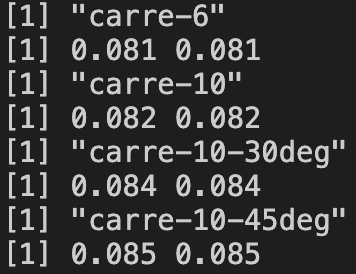
\includegraphics[height=5cm]{squares_main_moments.png}
    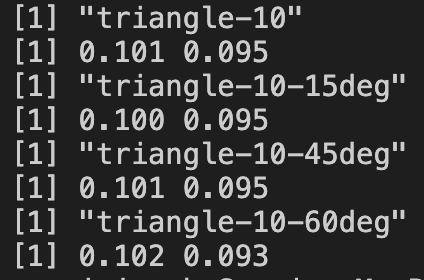
\includegraphics[height=5cm]{triangles_main_moments.png}
    \caption{Main inertia moments}
    \label{fig:main_inertia_moments}
\end{figure}

\subsection{Main axis of inertia}
\paragraph{}
The \emph{eigen vectors} of the $I$ matrix can tell us how the shapes are oriented.
We can clearly see that the 2 squares that are not rotated have the same \emph{eigen vectors}. The triangles, however, all have different vectors because they are all rotated in a different way, but their \emph{main moments of inertia} are the same.

\begin{figure}[h]
    \centering
    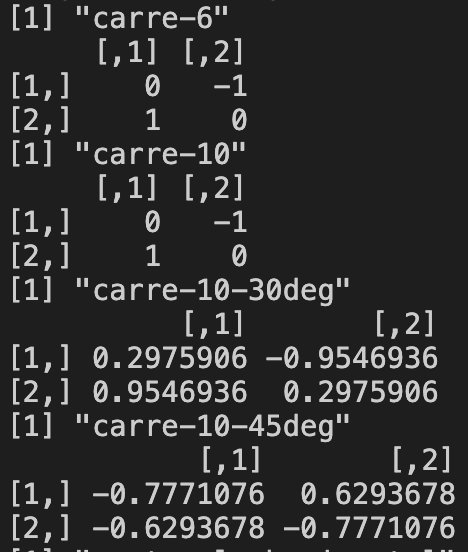
\includegraphics[height=5cm]{squares_main_axis.png}
    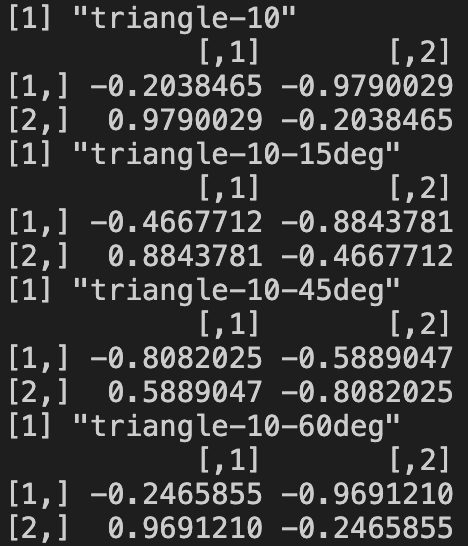
\includegraphics[height=5cm]{triangles_main_axis.png}
    \caption{Main inertia axis}
    \label{fig:main_inertia_axis}
\end{figure}


\paragraph{}
Having made these observation, we can conclude that these attributes are fairly important to describe a shape. They can tell us how their ``weight'' is distributed over their \emph{main axis of inertia}.

\clearpage

\section{Hu invariants}
\paragraph{}
Using the \emph{normalised center moments}, we can define the \emph{Hu invariants}. These are invariants with respect to translation, scale, and rotation.
Please refer to NANNANANANA for more information.
\paragraph{}
Analysing the invariants, we can see that...